\section{Compact RCNN architecture}
\label{sec:rcnn}

The overview of workflow within the RCNN architecture is displayed in Fig.~\ref{fig:RCNN-layout}. After measuring $r$ rounds of stabilizers and translating them to $r+1$ time steps of detector events, the NN redistributes these inputs spatially into the strides of each kernel type and also groups them temporally for the different temporal stages of the architecture. The different temporal stages are shown in Fig.~\ref{fig:RCNN-layer-prog} and are divided as an initial stage, a lead-in stage for recurrence, a true recurrent stage, and a final stage, each handled by their own NN layers and unique sets of parameters. The initial and final layers examine the first and last two rounds of stabilizer measurements, respectively, whereas the lead-in and recurrent layers examine three rounds at a time.

Each of the temporal layers start with the evaluation of all kernel strides, followed by the combination of kernel outputs. All temporal layers share the same base class, and they are differentiated by the nuances in kernel evaluation steps. Except for the initial state kernel, all kernels receive the initial error states of the data qubits that are included in a stride, and the error states from the last round if those are distinct from the initial states. The passed error states are those evaluated from the full temporal layer (denoted with $z^{\,\prime\prime}$ in Fig.~\ref{fig:RCNN-layout}), not the error states from the corresponding kernel strides from previous rounds (denoted with.$x^{\,\prime}$ in Fig.~\ref{fig:RCNN-layout}). While the implementation of the lead-in and recurrent kernel layers is through the same base class in the architecture, we separate them conceptually given that only the recurrent kernel layer can access at least two distinct prior data qubit error states, whereas in the lead-in kernel layer, the output of the initial temporal layer serves as the only unique prior error state that can be passed.

The output of temporal layers is passed through the same decoder layer, which is responsible for decoding the $z$-like error states over the data qubits at each round into the probability of an error over the chosen logical observable (or the probability space over the chosen observables). 
In the current architecture, the decoder layer consists of $d^2$ $z$-like inputs, mapped first to a pair of hidden dense layers with bias parameters and ReLU activation, and then to the output probability space through a sigmoid activation and, again, with a set of bias parameters. For the hidden layers, our tests at $d=5$ suggest 100 nodes to be a reasonable size for each, but rigorous tests for the dependence of the number of hidden layer nodes to $d$ should be performed in future studies. While separate decoder layers could be conceived for each temporal layer type, we have not found any significant improvement in round-by-round and final accuracy levels by constructing independent decoder layers.

\begin{figure*}[htb]
\centering
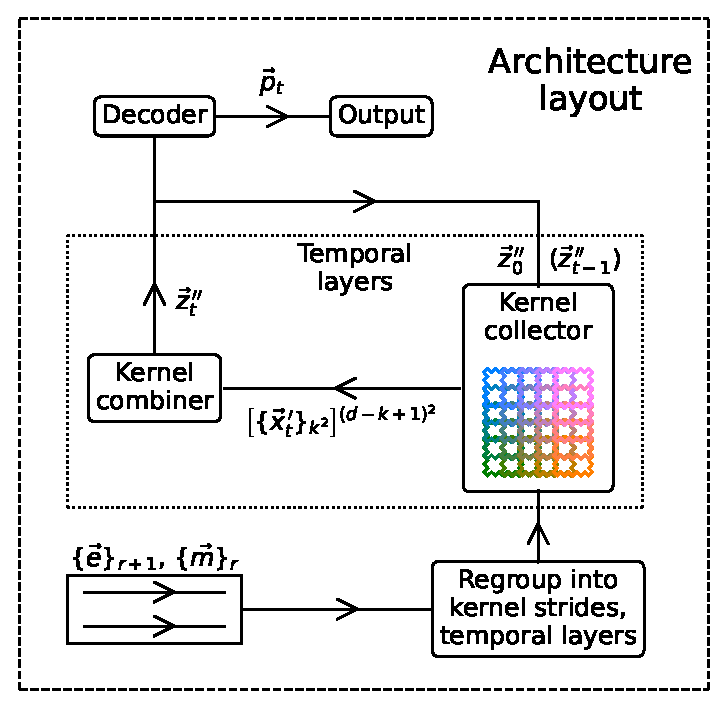
\includegraphics[width=0.9\textwidth]{general_architecture_layout.pdf}
\ccaption
{Layout of the compact RCNN architecture}
{
The inputs to the compact RCNN workflow are the stabilizer measurements from $r$ rounds, $\vec{m}$, and associated $r+1$ rounds of detector events, $\vec{e}$, which are displayed at the bottom left corner, with the vector notation representing qubit positions, and the subscripts in curly braces representing the temporal dimensionality.
The inputs are regrouped into kernels based on the spatial positions of the measure qubits and are fed sequentially into the layers of the NN, enclosed in dotted lines, that define the recurrent time evolution of the error state of the surface code. Each temporal layer consists of its own instances of a kernel collector, which is responsible for constructing the unique kernel types and traversing the entire surface code with them, and a kernel combiner, which is responsible for constructing a separate rule instance to combine the $x$-like evaluation results of the kernels (a list of $(d-k+1)^2$ number of $k^2$-dimensional vectors) into a $d^2$ array of $z$-like results. The output of the kernel combiner defines a multidimensional error state for the temporal slice and is fed into the next temporal slice as the last known (or initial) state. It can also be decoded through a decoder layer to produce a vector of probabilities for the logical observables of the circuit. As used throughout the paper, singly-primed variables denote the outputs of the kernels, and doubly-primed variables denote the outputs of the kernel combiner.
}
\label{fig:RCNN-layout}
\end{figure*}

%%%%%%%%%%%%%%%%%%%%%%%%%%%%%
\begin{figure*}[htb]
\centering
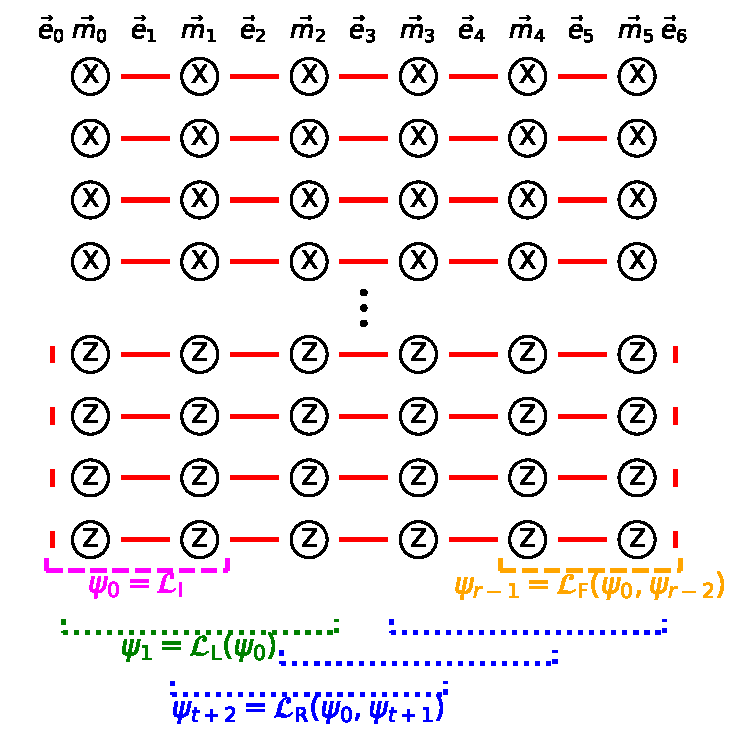
\includegraphics[width=0.9\textwidth]{RCNN_layer_progression_d3_r6.pdf}
\ccaption
{Temporal progression of the recurrent NN architecture}
{
Illustrated is the temporal progression for a memory experiment over the logical $Z_L$ observable in an arbitrary distance-$d$ surface code with $r=6$ rounds. Each column of circles marks a different stabilizer measurement round, with the circles corresponding to the readings from the $X$ or $Z$ measure qubits, $\vec{m}_t$ for $0\leq t \leq r-1$. The horizontal red lines mark \type{C} detector events, $\vec{e}_t$ for $1 \leq t \leq r-1$, and the vertical red lines next to the $Z$ measure qubit readings mark \type{S} detector events at the beginning, $\vec{e}_0$, and the end of the memory experiment, $\vec{e}_{r}$.
Each bracket at the bottom corresponds to a different pass in the recurrent architecture, with the extent of the brackets demarcating the measure qubit readings and detector events that are used as input features.
The initialization layer, $\mathcal{L}_I$ (magenta), provides an initial error state $\vec{z}^{\,\prime\prime}_0$ from $\vec{m}_0$, $\vec{m}_1$, $\vec{e}_0$, and $\vec{e}_1$.
The lead-in layer, $\mathcal{L}_L$ (green), updates the error state to $\vec{z}^{\,\prime\prime}_1$ using the first available triplet stabilizer state parametrization from $\vec{m}_{0 \text{---} 2}$, $\vec{e}_1$ and $\vec{e}_2$, and the state $\vec{z}^{\,\prime\prime}_0$.
The recurrent layer, $\mathcal{L}_R$ (blue), then strides through the rest of rounds one by one: To obtain each error state update $\vec{z}^{\,\prime\prime}_{t}$ ($t\geq2$), this layer uses the triplet stabilizer state parametrization from $\vec{m}_{(t-1) \text{---} (t+1)}$, $\vec{e}_{t}$ and $\vec{e}_{t+1}$, the previous error state $\vec{z}^{\,\prime\prime}_{t-1}$, and the initial error state $\vec{z}^{\,\prime\prime}_{0}$.
At the end, the finalization layer, $\mathcal{L}_F$ (orange), provides the final error state prediction $\vec{z}^{\,\prime\prime}_{r-1}$ upon receiving $\vec{m}_{r-2}$ and $\vec{m}_{r-1}$, $\vec{e}_{r-1}$ and $\vec{e}_r$, and the last known error state $\vec{z}^{\,\prime\prime}_{r-2}$ and the initial error state $\vec{z}^{\,\prime\prime}_{0}$.
}
\label{fig:RCNN-layer-prog}
\end{figure*}
%%%%%%%%%%%%%%%%%%%%%%%%%%%%%


The initial state kernel layer is the simplest in structure. As illustrated in Fig.~\ref{fig:RCNN-init-arch}, the stabilizer measurements and detector events are passed through stabilizer measurement and detector event embedders discussed in Section~\ref{sec:kernels-r2}, respectively. 
The quadratic representation of the inputs are then passed through separate dense layers with no bias and same output dimensions so that they can be added element-wise -- one should note that this approach is equivalent to having a single dense layer with no bias over the union of the outputs of the embedding layers. 
The final set of $z$-like pre-combination error states are exponentiated and passed into the combination step of the initial temporal layer.


%%%%%%%%%%%%%%%%%%%%%%%%%%%%%
\begin{figure*}[htb]
\centering
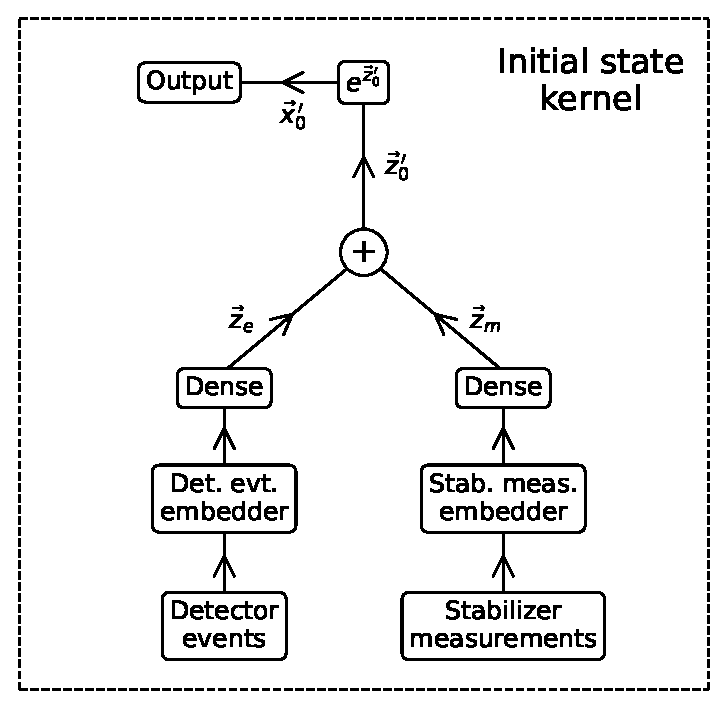
\includegraphics[width=0.6\textwidth]{initial_state_kernel_architecture.pdf}
\ccaption
{Initial state kernel architecture}
{
The detector events and stabilizer measurements that pertain to each kernel stride pass through embedder layers that convert linear or quadratic representations of the bits into values between -1 and 1.
The output of the embedders pass through dense layers with no bias term to convert them to $z$-like vectors of $k^2$ elements, and the two vectors are added. The final result of the kernel is returned as $x$-like values after element-wise exponentiation.
}
\label{fig:RCNN-init-arch}
\end{figure*}
%%%%%%%%%%%%%%%%%%%%%%%%%%%%%

As mentioned before, all kernel layers except the initial state kernel account for a set of prior states from the full temporal layer evaluation. This is accomplished through a state correlator layer architecture, illustrated in Fig.~\ref{fig:RCNN-state-corr}. The state correlator first converts the $z$-like input states from $n$ time steps, including the $z$-like states that result from the combination of dense layers in each kernel, into $n$ $\vec{\alpha}$-variables, $n-1$ $\vec{f}$-variables, and $n(n-1)/2$ $\vec{c}_\varphi$-variables. 
In this notation, the vector indices run over the data qubits of the kernel, and each of these sets of variables are determined through transformations of $z$-like underlying variables, parametrized linearly over the passed $z$-like states, with trainable weights initialized before training to 0, and trainable bias parameters initialized at 1. 
The $\alpha$-variables, bounded between -1 and 1, act as sign reversion indicators over the input states. 
After transforming the products $\vec{\alpha} \cdot \vec{z}$ using the exponential function into $x$-like values, we combine them using the $\vec{f}$ fractions and the $\vec{c}_\varphi$ phase factors in a way algebraically similar to the combination of kernel outputs described in Section~\ref{sec:kerncomb}. The final $x$-like outputs of the state correlator constitute the outputs of the kernel that maintains the correlator as well.


%%%%%%%%%%%%%%%%%%%%%%%%%%%%%
\begin{figure*}[htb]
\centering
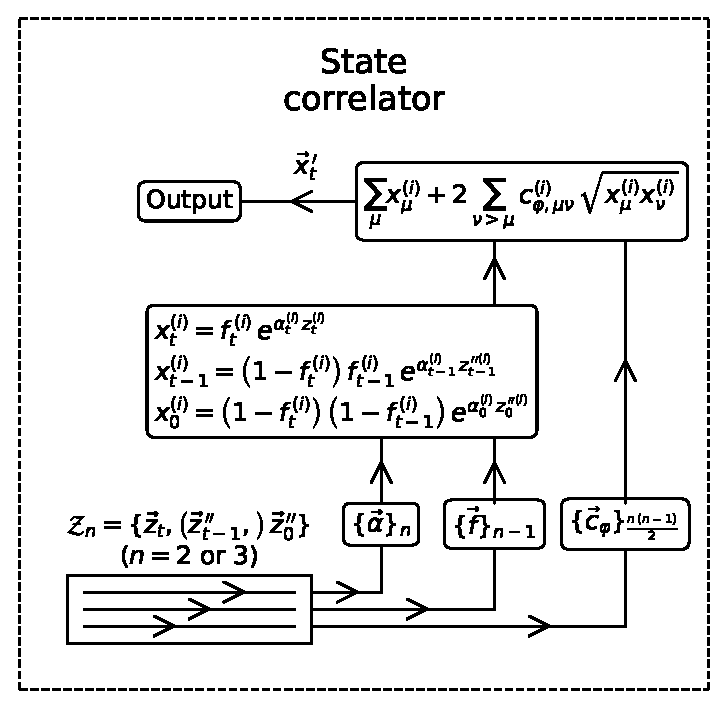
\includegraphics[width=0.6\textwidth]{state_correlator_architecture.pdf}
\ccaption
{State correlator architecture}
{
The inputs to the correlator are the kernel state prediction at current time, the state prediction from the initial temporal layer, and, if distinct from the initial state, the state prediction from the temporal layer for the previous round. 
For each input state, the values $\vec{\alpha}$ with $\abs{\alpha}<1$ are parametrized through a $\mathrm{tanh}(\vec{z}_\alpha)$ transformation such that $\vec{z}_\alpha$ depends linearly on the input states, along with a constant term. The set of $\vec{f}$ values that define recursive fractions for the states are also found in a similar way, but with a sigmoid transformation instead to keep the fractions bounded between 0 and 1. 
The phase terms $\vec{c}_\varphi$ between the states are constructed with a similar hyperbolic tangent transformation, independent of $\vec{\alpha}$. 
The vectors $\vec{\alpha}$ and $\vec{f}$ are used to compute $x$-like variables for each time step, with the sign of each $\alpha$ signifying whether the error probability that could be obtained by the corresponding state should be inverted or not. One can then combine the computed $x$-like variables as absolute values of complex numbers with phase differences using $\vec{c}_\varphi$ to obtain a final $x$-like vector. In the illustrated mathematical expressions, the superscript $(i)$ signifies element-wise operations, and the Greek-letter indices $\mu$ and $\nu$ are used in the $x$-like variable summation over the time steps.
}
\label{fig:RCNN-state-corr}
\end{figure*}
%%%%%%%%%%%%%%%%%%%%%%%%%%%%%


Because they feature state correlator layers, the lead-in, recurrent, and final state kernels are structurally similar to each other. 
The flowcharts of the lead-in and recurrent kernel layers are displayed in Fig.~\ref{fig:RCNN-lirec-arch}, whereas that of the final state kernel is displayed in Fig.~\ref{fig:RCNN-final-arch}.
The only differences between the base class of the lead-in and recurrent state kernels, and the class for the final state kernel, are the number of rounds processed as input, and the fact that the special detector events at the end of the full QEC cycle are also passed to the final state kernels.
These differences lead to the choices to utilize the triplet state probability embedder layer in lead-in and recurrent layers, and the stabilizer measurement embedder layer in the final state kernel for the quadratic representation of the stabilizer measurements.


%%%%%%%%%%%%%%%%%%%%%%%%%%%%%
\begin{figure*}[htb]
\centering
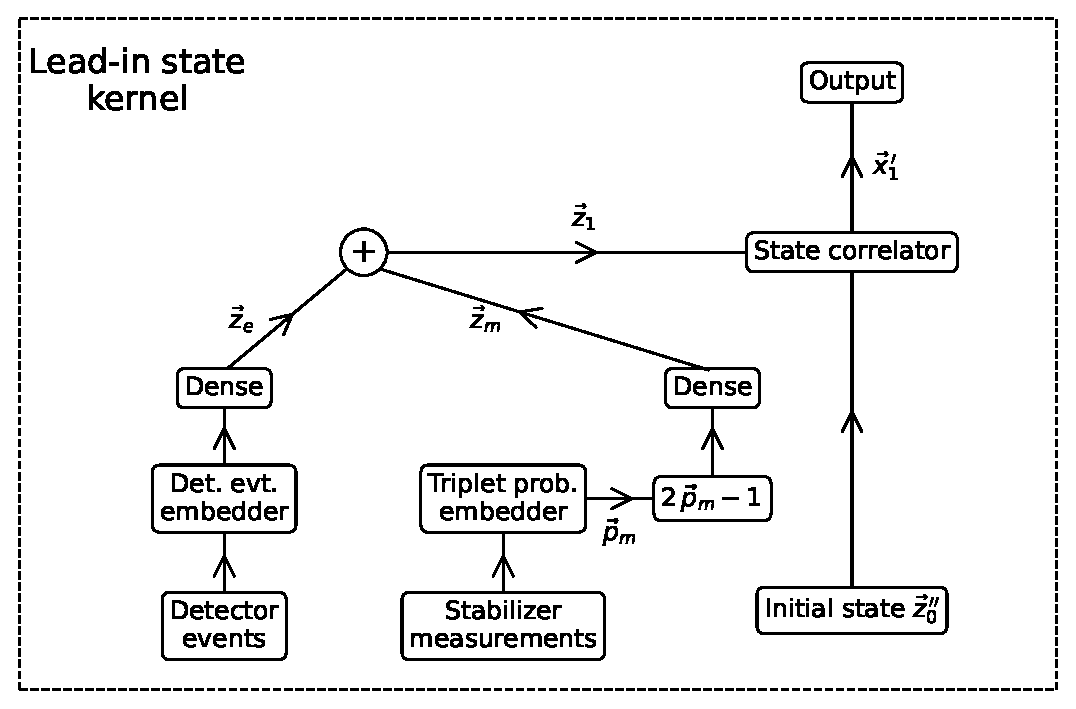
\includegraphics[width=0.9\textwidth]{leadin_state_kernel_architecture.pdf}\\
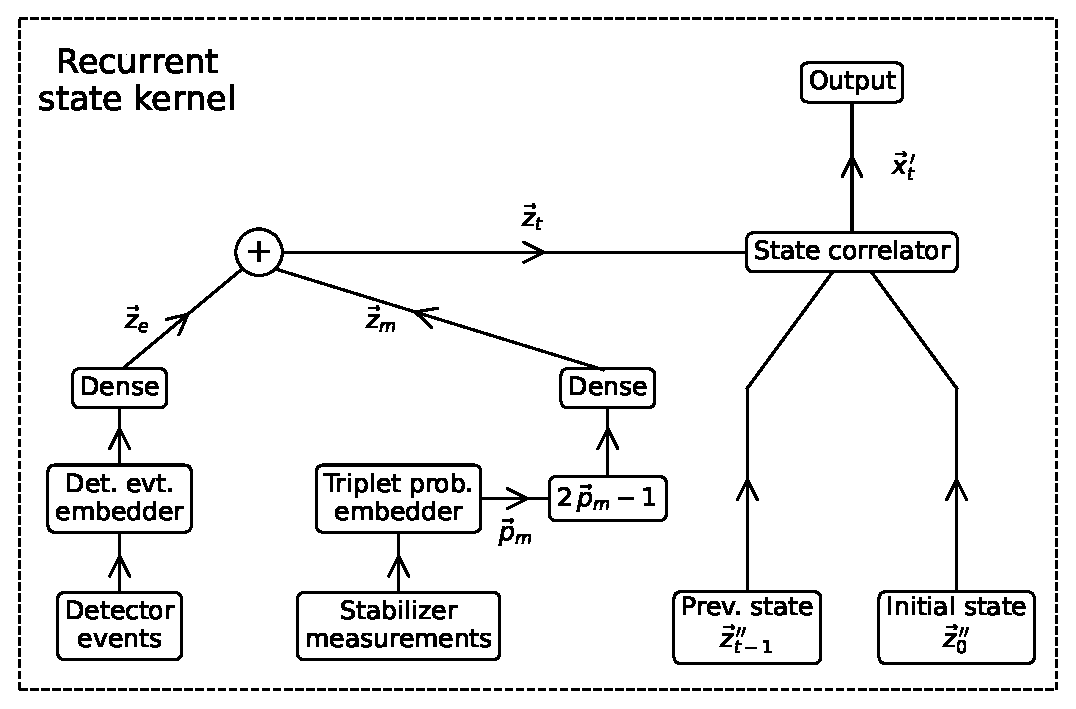
\includegraphics[width=0.9\textwidth]{recurrent_state_kernel_architecture.pdf}
\ccaption
{Lead-in and recurrent state kernel architectures}
{
Lead-in state kernel, top: The detector events that pertain to each kernel stride pass through an embedder layer that converts linear or quadratic representations of the bits into values between -1 and 1, and these values are then passed through a dense layer with no bias term. Similarly, stabilizer measurements are passed through a triplet stat probability embedder, and the probabilities are transformed linearly into values between -1 and 1 before passing through a similar dense layer.
The $z$-like results of the two dense layers, each being vectors of $k^2$ elements, are summed, and together with the initial states of the data qubits corresponding to the kernel window, they are passed to a state correlator. The correlator produces the final $x$-like output of the lead-in layer.
Recurrent state kernel, bottom: The architecture is almost exactly the same as that of the lead-in state. The only difference is that the recurrent state kernel passes both the previous and the initial state of the data qubits within the kernel window to the state correlator.
}
\label{fig:RCNN-lirec-arch}
\end{figure*}
%%%%%%%%%%%%%%%%%%%%%%%%%%%%%



%%%%%%%%%%%%%%%%%%%%%%%%%%%%%
\begin{figure*}[htb]
\centering
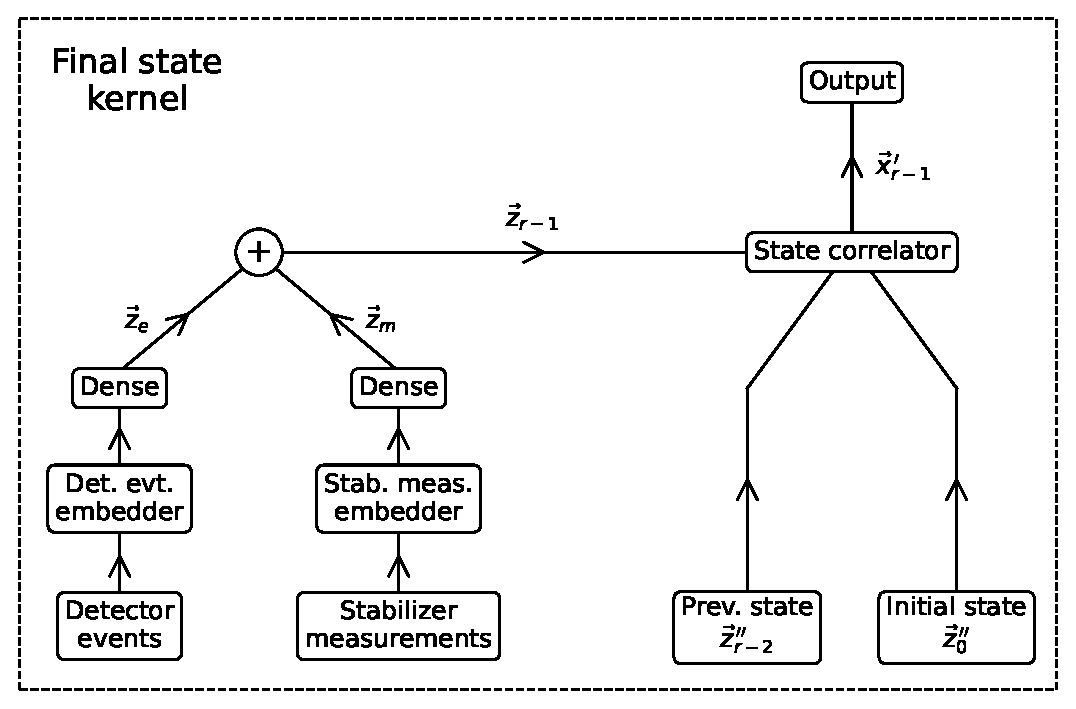
\includegraphics[width=0.9\textwidth]{final_state_kernel_architecture.pdf}
\ccaption
{Final state kernel architectures}
{
The detector events and stabilizer measurements that pertain to each kernel stride pass through embedder layers that convert linear or quadratic representations of the bits into values between -1 and 1.
The output of the embedders pass through dense layers with no bias term to convert them to $z$-like vectors of $k^2$ elements, and the two vectors are added.
Together with the initial and last states of the data qubits corresponding to the kernel window, the summed vector is passed to a state correlator, and the correlator produces the final $x$-like output of this layer.
When there are only two rounds in a QEC cycle, the initial and last states are identical, so the implementation passes only one prior state.
}
\label{fig:RCNN-final-arch}
\end{figure*}
%%%%%%%%%%%%%%%%%%%%%%%%%%%%%


In determining the final probability of logical observable errors, the architecture provides the option to run in two different modes:
\begin{itemize}
\item In standard mode, the architecture determines a probability value for either all rounds requested, or a certain number of specified rounds, including the last round. If a valid cutoff round is specified, even if it is the last round, we define this prediction as an early stopping condition and do not run the final temporal layer. 
Otherwise, the predictions are produced after adding the final temporal layer.
\item In per-round prediction mode, the architecture determines a probability value for each round in the QEC cycle except for the first one, which is consumed by the initial temporal layer for reliable warmup without any corresponding output. This option is useful if one would like to train the NN over a shorter cycle that covers each temporal layer and reuse it for longer ones.
\end{itemize}
Ultimately, the specific use case would dictate how the architecture is trained and utilized, so we leave it to the user to decide which mode suits their needs best.
